% !TeX program = lualatex
% allgem. Dokumentenformat
\documentclass[a4paper,12pt,headsepline]{scrartcl}
%Variablen welche innerhalb der gesamten Arbeit zur Verfügung stehen sollen
\newcommand{\titleDocument}{Bachelorarbeit}
\newcommand{\subjectDocument}{im Studiengang Informatik}

% weitere Pakete
% Grafiken aus PNG Dateien einbinden
\usepackage{graphicx}

% Deutsche Sonderzeichen benutzen 
\usepackage{ngerman}

% deutsche Silbentrennung
\usepackage[ngerman]{babel}
\usepackage{amsmath}

% Eurozeichen einbinden
\usepackage[right]{eurosym}

% Umlaute unter UTF8 nutzen
\usepackage[utf8]{inputenc}

% Zeichenencoding
\usepackage[T1]{fontenc}

\usepackage{lmodern}
\usepackage{fix-cm}

% floatende Bilder ermöglichen
%\usepackage{floatflt}
\usepackage{tikz}
    \usetikzlibrary{positioning}
    
    \tikzset{basic/.style={draw,fill=blue!20,text width=1em,text badly centered}}
    \tikzset{input/.style={basic,circle}}
    \tikzset{weights/.style={basic,rectangle}}
    \tikzset{functions/.style={basic,circle,fill=blue!10}}
% mehrseitige Tabellen ermöglichen
\usepackage{longtable}
\usetikzlibrary{graphdrawing}
\usetikzlibrary{graphs}
\usegdlibrary{trees}
% Unterstützung für Schriftarten
%\newcommand{\changefont}[3]{ 
%\fontfamily{#1} \fontseries{#2} \fontshape{#3} \selectfont}

% Packet für Seitenrandabständex und Einstellung für Seitenränder
\usepackage{geometry}
\geometry{left=3.5cm, right=2cm, top=2.5cm, bottom=2cm}

% Paket für Boxen im Text
\usepackage{fancybox}

% bricht lange URLs "schoen" um
\usepackage[hyphens,obeyspaces,spaces]{url}

% Paket für Textfarben
\usepackage{color}

% Mathematische Symbole importieren
\usepackage{amssymb}

% auf jeder Seite eine Überschrift (alt, zentriert)
%\pagestyle{headings}

% erzeugt Inhaltsverzeichnis mit Querverweisen zu den Kapiteln (PDF Version)
\usepackage[bookmarksnumbered,pdftitle={\titleDocument},hyperfootnotes=false]{hyperref} 
%\hypersetup{colorlinks, citecolor=red, linkcolor=blue, urlcolor=black}
%\hypersetup{colorlinks, citecolor=black, linkcolor= black, urlcolor=black}

% neue Kopfzeilen mit fancypaket
\usepackage{fancyhdr} %Paket laden
\pagestyle{fancy} %eigener Seitenstil
\fancyhf{} %alle Kopf- und Fußzeilenfelder bereinigen
\fancyhead[L]{\nouppercase{\leftmark}} %Kopfzeile links
\fancyhead[C]{} %zentrierte Kopfzeile
\fancyhead[R]{\thepage} %Kopfzeile rechts
\renewcommand{\headrulewidth}{0.4pt} %obere Trennlinie
%\fancyfoot[C]{\thepage} %Seitennummer
%\renewcommand{\footrulewidth}{0.4pt} %untere Trennlinie

% für Tabellen
\usepackage{array}

% Runde Klammern für Zitate
%\usepackage[numbers,round]{natbib}

% Festlegung Art der Zitierung - Havardmethode: Abkuerzung Autor + Jahr
\bibliographystyle{alphadin}

% Schaltet den zusätzlichen Zwischenraum ab, den LaTeX normalerweise nach einem Satzzeichen einfügt.
\frenchspacing

% Paket für Zeilenabstand
\usepackage{setspace}

% für Bildbezeichner
\usepackage{capt-of}

% für Stichwortverzeichnis
\usepackage{makeidx}
\usepackage{pgfplots}

% für Listings
\usepackage{listings}
\lstset{numbers=left, numberstyle=\tiny, numbersep=5pt, keywordstyle=\color{black}\bfseries, stringstyle=\ttfamily,showstringspaces=false,basicstyle=\footnotesize,captionpos=b}
\lstset{language=java}

% Indexerstellung
\makeindex

% Abkürzungsverzeichnis
\usepackage[german]{nomencl}
\let\abbrev\nomenclature

% Abkürzungsverzeichnis LiveTex Version
\renewcommand{\nomname}{Abkürzungsverzeichnis}
\setlength{\nomlabelwidth}{.25\hsize}
\renewcommand{\nomlabel}[1]{#1 \dotfill}
\setlength{\nomitemsep}{-\parsep}
\makenomenclature
%\makeglossary


% Abkürzungsverzeichnis TeTEX Version
% \usepackage[german]{nomencl}
% \makenomenclature
% %\makeglossary
% \renewcommand{\nomname}{Abkürzungsverzeichnis}
% \setlength{\nomlabelwidth}{.25\hsize}
% \renewcommand{\nomlabel}[1]{#1 \dotfill}
% \setlength{\nomitemsep}{-\parsep}

% Disable single lines at the start of a paragraph (Schusterjungen)
\clubpenalty = 10000
% Disable single lines at the end of a paragraph (Hurenkinder)
\widowpenalty = 10000
\displaywidowpenalty = 10000

\begin{document}
% hier werden die Trennvorschläge inkludiert

%hier müssen alle Wörter rein, welche Latex von sich auch nicht korrekt trennt bzw. bei denen man die genaue Trennung vorgeben möchte
\hyphenation{
Film-pro-du-zen-ten
Lux-em-burg
Soft-ware-bau-steins
zeit-in-ten-siv
}

%Schriftart Helvetica
%\changefont{phv}{m}{n}

% Leere Seite am Anfang
\newpage
\thispagestyle{empty} % erzeugt Seite ohne Kopf- / Fusszeile
\section*{ }

% Titelseite %
% das Papierformat zuerst
%\documentclass[a4paper, 11pt]{article}

% deutsche Silbentrennung
%\usepackage[ngerman]{babel}

% wegen deutschen Umlauten
%\usepackage[ansinew]{inputenc}

% hier beginnt das Dokument
%\begin{document}


\thispagestyle{empty}

%\begin{figure}[t]
% \includegraphics[width=0.6\textwidth]{abb/fh_koeln_logo}
%\end{figure}

\begin{figure}[t]
 \centering
 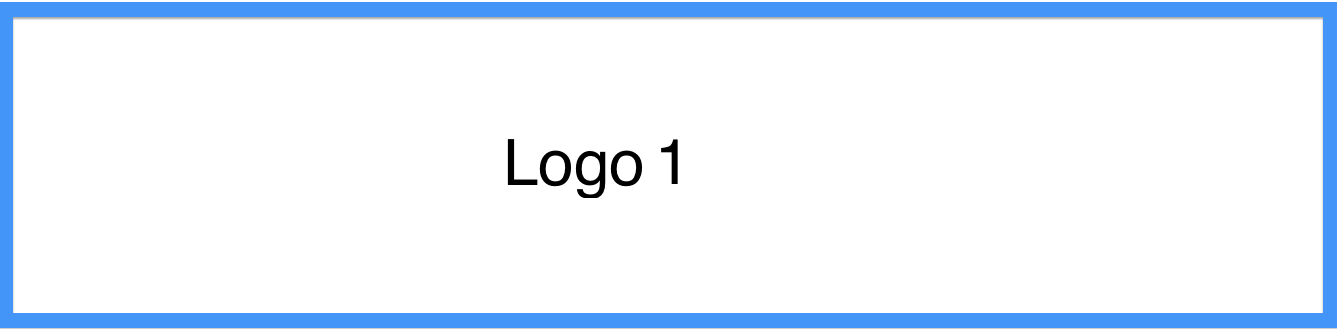
\includegraphics[width=0.6\textwidth]{abb/logo1}
~~~~~~~~~~
 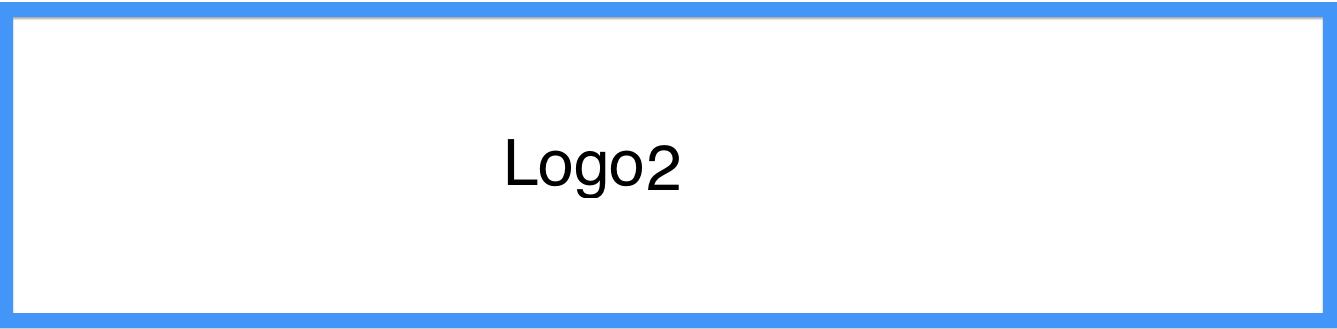
\includegraphics[width=0.3\textwidth]{abb/logo2}
\end{figure}


\begin{verbatim}


\end{verbatim}

\begin{center}
\Large{Goethe-Universität Frankfurt}\\

\end{center}


\begin{center}
\Large{Fachbereich 12 - Informatik und Mathematik}
\end{center}
\begin{verbatim}




\end{verbatim}
\begin{center}
\doublespacing
\textbf{\LARGE{\titleDocument}}\\
\singlespacing
\begin{verbatim}

\end{verbatim}

\end{center}
\begin{verbatim}

\end{verbatim}
\begin{center}

\end{center}
\begin{verbatim}

\end{verbatim}
\begin{center}
\textbf{zur Erlangung des akademischen Grades \\ Bachelor of Science}
\end{center}
\begin{verbatim}






\end{verbatim}
\begin{flushleft}
\begin{tabular}{llll}
\textbf{Thema:} & & Deep Neural Networks for occluded Image Recognition & \\
& & \\
\textbf{Autor:} & & Julius Taylor <s8423760@stud.uni-frankfurt.de>& \\
& & MatNr. 5210444 & \\
& & \\
\textbf{Version vom:} & & \today &\\
& & \\
\textbf{Betreuer:} & & Prof. Dr. Jochen Triesch &\\
\end{tabular}
\end{flushleft}

% römische Numerierung
%\pagenumbering{arabic}

% 1.5 facher Zeilenabstand
\onehalfspacing

% Sperrvermerk
\section*{Sperrvermerk}
\textcolor{red}{
Die vorliegende Arbeit beinhaltet interne und vertrauliche Informationen der Firma <Firmenname>.
Die Weitergabe des Inhalts der Arbeit im Gesamten oder in Teilen sowie das Anfertigen
von Kopien oder Abschriften - auch in digitaler Form - sind grundsätzlich untersagt.
Ausnahmen bedürfen der schriftlichen Genehmigung der Firma <Firmenname>.
}

% Einleitung / Abstract
\section*{Zusammenfassung}
Convolutional Neural Networks sind haben in den letzten Jahren in vielen Machine Learning Problemen bisher ungeahnte Benchmarks ermöglicht, die in einigen Domänen sogar Menschliche Performance übersteigen. Dabei sind rekurrente Verbindungen in solchen Netzen bisher selten beachtet worden, obwohl die Struktur des menschlichen Gehirns solche nahelegt. In dieser Arbeit versuche ich die Ergebnisse von Spoerer und Kriegeskorte {} zu reproduzieren, welche Hinweise fanden, dass das Inkorporieren solcher rekurrenten Verbindungen Vorteile bei der Bilderkennung in schwierigen Szenarien, wie der teilweisen Verdeckung zu erkennender Objekte bieten kann.

\begin{verbatim}

like whaat?

\end{verbatim}

\section*{Abstract}


% einfacher Zeilenabstand
\singlespacing

% Inhaltsverzeichnis anzeigen
\newpage
\tableofcontents

% das Abbildungsverzeichnis
%\newpage
% Abbildungsverzeichnis soll im Inhaltsverzeichnis auftauchen
\addcontentsline{toc}{section}{Abbildungsverzeichnis}
% Abbildungsverzeichnis endgueltig anzeigen
\listoffigures

% das Tabellenverzeichnis
%\newpage
% Abbildungsverzeichnis soll im Inhaltsverzeichnis auftauchen
\addcontentsline{toc}{section}{Tabellenverzeichnis}
% \fancyhead[L]{Abbildungsverzeichnis / Abkürzungsverzeichnis} %Kopfzeile links
% Abbildungsverzeichnis endgueltig anzeigen
\listoftables

%% WORKAROUND für Listings
%\makeatletter% --> De-TeX-FAQ
%\renewcommand*{\lstlistoflistings}{%
%  \begingroup
%    \if@twocolumn
%      \@restonecoltrue\onecolumn
%    \else
%      \@restonecolfalse
%    \fi
%    \lol@heading
%    \setlength{\parskip}{\z@}%
%    \setlength{\parindent}{\z@}%
%    \setlength{\parfillskip}{\z@ \@plus 1fil}%
%    \@starttoc{lol}%
%    \if@restonecol\twocolumn\fi
%  \endgroup
%}
%\makeatother% --> \makeatletter
% das Listingverzeichnis
%\newpage
% Listingverzeichnis soll im Inhaltsverzeichnis auftauchen
\addcontentsline{toc}{section}{Listingverzeichnis}
\fancyhead[L]{Abbildungs- / Tabellen- / Listingverzeichnis} %Kopfzeile links
\renewcommand{\lstlistlistingname}{Listingverzeichnis}
\lstlistoflistings
%%%%

% das Abkürzungsverzeichnis
%\newpage
% Abkürzungsverzeichnis soll im Inhaltsverzeichnis auftauchen
\addcontentsline{toc}{section}{Abkürzungsverzeichnis}
% das Abkürzungsverzeichnis entgültige Ausgeben
\fancyhead[L]{Abkürzungsverzeichnis} %Kopfzeile links
\nomenclature{UGC}{User Generated Content}
\nomenclature{CSS}{Cascading Style Sheets}
\nomenclature{JS}{JavaScript}
\nomenclature{SQL}{Structured Query Language}
\nomenclature{GPL}{GNU General Public License}
\nomenclature{GNU}{GNU is not Unix}
\nomenclature{LGPL}{GNU Lesser General Public License}
\nomenclature{XMPP}{Extensible Messaging and Presence Protocol}
\nomenclature{IM}{Instant Message}
\nomenclature{CMS}{Content Management System}
\nomenclature{RSS}{Really Simple Syndication}
\nomenclature{JSON}{JavaScript Object Notation}
\nomenclature{HTML}{Hypertext Markup Language}
\nomenclature{TDD}{Test-driven development}
\nomenclature{GUI}{Graphical User Interface}
\nomenclature{KPI}{Key Performance Indicator}
\nomenclature{WWW}{World Wide Web}
\nomenclature{OCR}{Optical Character Recognition}
\nomenclature{ERM}{Entity Relationship Modell}

\printnomenclature

% Definiert Stegbreite bei zweispaltigem Layout
\setlength{\columnsep}{25pt}

\newpage
\fancyhead[L]{\nouppercase{\leftmark}} %Kopfzeile links

% 1,5 facher Zeilenabstand
\onehalfspacing

% einzelne Kapitel
\section{Einleitung}\label{einleitung}

\section{Background}
\subsection{Supervised Learning}
\newcommand\yhat{\,\hat{y}}
\newcommand\Yhat{\, \hat{Y}}

The common ground for all further aspects in this work will be supervised learning, which is most generally speaking simply the task of deriving a function from data. This function should be able to map given inputs or data points to some sort of output. In the supervised setting, data is given with an associative label such, that the inferred function is able to map said input data to the correct labels, without explicitly looking at the given labels. The learning algorithm, when deriving said function, therefore has to use patterns and structure among the data points to learn something about the quality of a given data point. Outputs are generally either of a quantitative type e.g. temperature measurements or changes in stock price or of a qualitative type like distinctive types of flowers. Tasks involving the former kinds of outputs are generally referred to as regression problems whereas the tasks involving the latter are generally called classification problems.
\\We can roughly articulate the supervised learning problem as follows: for a given input $X$, an associated label $Y$ and a function $ \mathbb{F}(X)= \Yhat$, $\mathbb{F}$ makes a good prediction, when $\Yhat$ is close to $Y$. Proximity, in this case, must be defined and can vary depending on the type of data which is present. For a regression problem of e.g. predicting tomorrows temperature, the prediction is better, the more similar the predicted value $\Yhat$ and tomorrows true temperature are, measured by the absolute distance of $|Y-\Yhat|$.
X in this case could be a vector of meteorologic measurements which are regarded highly predictive of short term weather prognosis.
\subsubsection{Linear Models}
Linear Regression has been a staple in statistics and machine learning and remains a very important and widely used tool \cite{hastie01statisticallearning}. As it serves as the basis for a wide range of more complex machine learning algorithms like logistic regression and in some sense even Deep Neural Networks, it serves as a good introduction. The linear model 
\begin{align*}
	\mathbb{F}(X) =  \beta + \sum_{i=1}^{|X|}w_ix_i = \yhat
\end{align*} 
predicts Y by using a linear combination of all input variables $x_i$ using weights $w_i$. $\beta$ is the intercept of the linear decision boundary, often referred to as the bias. Since in this case we are modeling a scalar value, $\yhat$ is a single value, but can also be N-vector if we're predicting values of higher dimensionality. To get an idea how good our model is performing, we first need to come up with a way of measuring its prediction quality. The sum of squares is a widely used method and sums each squared difference between any predicted value $\yhat_i$ and its corresponding true value $y_i$. We define the sum of squared errors as $E$, a function of our parameters $\mathbb{W}$ which we then can minimize. Since it is a quadratic function, its minimum always exists but does not have to be unique.
\begin{align*}
	E(\mathbb{W}) = \frac{1}{2}\sum_{i=1}^{N}(\yhat_i - y_i)^2 =
	\frac{1}{2}\sum_{i=1}^{N}(\sum_{j=1}^{|X|}(w_ix_i + \beta) - y_i)^2
\end{align*}
Minimizing E($\mathbb{W})$ with respect to $\mathbb{W}$ yields:
\begin{align*}
	\frac{\delta E}{\delta \mathbb{W}} =  \left(\frac{\delta E}{\delta w_1 },...,\frac{\delta E}{\delta w_n }\right) = \left( \sum_{i=1}^{N}(\yhat_i - y_i)x_1,...,\sum_{i=1}^{N}(\yhat_i - y_i)x_n \right)
\end{align*}

\subsection{Neuronale Netze}
Neuronale Netze sind biologisch inspirierte Programmierparadigma, welche es erlauben, iterativ vom Betrachten von Daten zu lernen. Dazu benötigen sie meist kein domänenspezifisches Wissen, sondern "lernen" Strukturen in den betrachteten Daten selbst zu erkennen. Die Grundeinheit solcher Netzwerke sind dabei künstliche Neuronen, die in Schichten angeordnet sind. Ein Neuron erhält eine Eingabe und propagiert sie über eine Verbindung (Synapse) an andere Neuronen weiter. Typischerweise senden Neuronen ihre Eingabe entlang eines Pfades von der Eingabe zur Ausgabe und haben Gewichte, die bestimmen, wie viel des erhaltenen Signals an folgende Neuronen weitergegeben wird.\\
Die simpelste Form eines Neuronalen Netzes ist ein einfaches Perzeptron, welches 1958 von Frank Rosenblatt in \cite{rosenblatt1958perceptron} vorgestellt wurde. Dieses basiert auf einer McCulloch-Pitts-Zelle, einem rudimentären Modell einer Nervenzelle nach \cite{mcculloch1943logical}, enthält mehrere Eingaben und produziert eine einzige Ausgabe. Perzeptrons können prinzipiell aus mehreren Schichten solcher Zellen bestehen, die in Reihe geschaltet sind. Dabei gibt eine Zelle ihren berechneten Output an ein Neuron der nächsten Schichten weiter. Solche Netzwerke heißen Multi-Layer-Perzeptron, im weiteren beschäftigen wir uns jedoch mit einer einzigen Zelle.
\begin{figure}[!h]
	\centering
	\begin{tikzpicture}
	\node[functions] (center) {f};
	\node[below of=center,font=\scriptsize,text width=4em]{};
	\node[right of=center] (right) {};
	\path[draw,->] (center) -- (right);
	\node[functions,left=3em of center] (left) {$\sum$};
	\path[draw,->] (left) -- (center);
	\node[weights,left=3em of left] (2) {$w_3$} -- (2) node[input,left of=2] (l2) {$x_3$};
	\path[draw,->] (l2) -- (2);
	\path[draw,->] (2) -- (left);
	\node[below of=2] (dots) {$\vdots$} -- (dots) node[left of=dots] (ldots) {$\vdots$};
	\node[weights,below of=dots] (n) {$w_n$} -- (n) node[input,left of=n] (ln) {$x_n$};
	\path[draw,->] (ln) -- (n);
	\path[draw,->] (n) -- (left);
	\node[weights,above of=2] (1) {$w_2$} -- (1) node[input,left of=1] (l1) {$x_2$};
	\path[draw,->] (l1) -- (1);
	\path[draw,->] (1) -- (left);
	\node[weights,above of=1] (0) {$w_1$} -- (0) node[input,left of=0] (l0) {$x_1$};
	\path[draw,->] (l0) -- (0);
	\path[draw,->] (0) -- (left);
	\node[below of=ln,font=\scriptsize] {Input};
	\node[below of=n,font=\scriptsize] {Gewichte};
	\end{tikzpicture}
	\caption{Ein einfaches Perzeptron mit n Eingängen}
\end{figure}
Das einfache, in Abbildung 1 dargestellte Perzeptron erhält n Eingänge $x_1,...,x_n \in \mathbb{R}$, die jeweils mit korrespondierenden Gewichten $w_1,...,w_n \in \mathbb{R}$ multipliziert werden. Die Summer der Gewichteten Eingänge wird dann als Argument der Aktivierungsfunktion verwendet. Die Ausgabe des Perzeptron lässt sich als eine Funktion seiner Eingaben wie folgt beschreiben:
\begin{align*}
	\mathbb{P}(\boldsymbol{x}, \boldsymbol{w}) = f(\sum_{i=1}^{n}w_ix_i)
\end{align*}
mit der Aktivierungsfunktion
\begin{align*}
	f(x) = \begin{cases} 1 &\mbox{if } x \geq 0 \\ 
	0 & \mbox{if } x < 0 \end{cases} 
\end{align*}
womit die Ausgabe als Zugehörigkeit zu einer klasse, entweder 0 oder 1 zu interpretieren ist.
\subsection{Convolutional Neural Networks}
\subsection{Recurrent Neural Networks}
\subsection{Unrolling Recurrent Netowrks}
\subsection{Backpropagation}
Backpropagation is a widely used technique to train neural networks. It is, in fact, the algorithm that made training deep neural networks tractable in the first place. While being originally introduced in the 1970's it has not been adapted until David Rumelheart, Geoffrey Hinton and Ronald Williams drew a lot of attention to it in their famous 1986 Paper \cite{rumelhart1988learning}. At the core of Backpropagation stand partial derivatives like $\frac{\delta C}{\delta w}$ of a cost function C with respect to a weight w. This gradient expresses, at what rate C changes if we tune w. Knowing how the error of the network behaves when changing a parameter can be very helpful, since we then can adjust it in a way, such that our total error decreases.
In order to minimize our cost function we therefore have to compute the partial derivatives of the networks cost function with regard to every variable in the network i.e. every weight and bias. We then use those gradients to move "downwards" on our cost function i.e. adding a small positive value to our weight or bias, if the gradient is negative and vice versa adding a small negative value, if the gradient is positive.
\\
\begin{tikzpicture}[>=stealth, every node/.style={circle, draw, minimum size=0.75cm}]
\graph [tree layout, grow=down, fresh nodes, level distance=0.5in, sibling distance=0.5in]
{
	g = e * f <- { 
		e = a + b <- { a, b },
		f = 3 * c <- { c }
	} 
};
\end{tikzpicture}

\section{Kapitel 1}\label{kapitel1}

\section{Kapitel 2}\label{kapitel2}

%....

\section{Diskussion}\label{Diskussion}

\section{Fazit}\label{fazit}



\onecolumn
% einfacher Zeilenabstand
\singlespacing
% Literaturliste soll im Inhaltsverzeichnis auftauchen
\newpage
\addcontentsline{toc}{section}{Literaturverzeichnis}
% Literaturverzeichnis anzeigen
\renewcommand\refname{Literaturverzeichnis}
\bibliography{Hauptdatei}

%% Index soll Stichwortverzeichnis heissen
% \newpage
% % Stichwortverzeichnis soll im Inhaltsverzeichnis auftauchen
% \addcontentsline{toc}{section}{Stichwortverzeichnis}
% \renewcommand{\indexname}{Stichwortverzeichnis}
% % Stichwortverzeichnis endgueltig anzeigen
% \printindex

\onehalfspacing
% evtl. Anhang
\newpage
\addcontentsline{toc}{section}{Anhang}
\fancyhead[L]{Anhang} %Kopfzeile links
\subsection*{Anhang}\label{anhang}


% Eidesstattliche Erklärung
\addcontentsline{toc}{section}{Eidesstattliche Erklärung}
\section*{Eidesstattliche Erklärung}
\thispagestyle{empty}

\begin{verbatim}

\end{verbatim}

\begin{LARGE}Eidesstattliche Erklärung zur <-Arbeit>\end{LARGE}
\begin{verbatim}


\end{verbatim}
Ich versichere, die von mir vorgelegte Arbeit selbstständig verfasst zu haben. Alle Stellen, die wörtlich oder sinngemäß aus veröffentlichten oder nicht veröffentlichten Arbeiten anderer entnommen sind, habe ich als entnommen kenntlich gemacht. Sämtliche Quellen und Hilfsmittel, die ich für die Arbeit benutzt habe, sind angegeben. Die Arbeit hat mit gleichem Inhalt bzw. in wesentlichen Teilen noch keiner anderen Prüfungsbehörde vorgelegen.



\begin{displaymath}
% use packages: array
\begin{array}{ll}
Unterschrift:~~~~~~~~~~~~~~~~~~~~~~~~~~~~~~~~~~~~~~~~~~
& Ort, Datum:~~~~~~~~~~~~~~~~~~~~~~~~~~~~~~~~~~~~~~~~~~
\end{array}
\end{displaymath}


% leere Abschlussseite
\newpage
\thispagestyle{empty} % erzeugt Seite ohne Kopf- / Fusszeile
\section*{ }

\end{document}